\chapter{System zur Visualisierung akustischer Schmerz-Scores}


Das Ziel dieser Arbeit ist die Ableitung des Schmerz-Scores aus einem Audiosignal sowie die darauf folgende Visualisierung dieser Schmerz-Scores. Folgende Anforderungen werden an das System gestellt:
\begin{enumerate}
	\item Das System muss dazu in der Lage sein, aus den akustischen Eigenschaften des Weinens die Schmerz-Score abzuleiten
	\item Das System muss dazu in der Lage sein, die Schmer-Score zu visualiseren.
	\item Die Verarbeitungspipeline muss genug Flexibilität bieten, um beliebige Pain-Scores einzubinden. 
	\item Die Analyse muss auch bei nicht-optimalen akustischen Bedingungen Einsatzfähig sein.
	\item Die Methoden müssen kontinuierlich eingesetzt werden können. Das heißt, dass zu einem Analysezeitpunkt nur Informationen verwendet werden können, die nicht in der Zukunft liegen.
\end{enumerate}

Im folgenden wird ein Überblick über bereits verföffentlichte Ansätze zur Analyse von akustischen Signalen Neugeborener oder sonstiger automatisierter Systeme zur Ableitung der Pain-Score gegeben.

\section{Literatur-Übeblick}
\label{sec:system_literature}

Bei der Aufgabenstellung handelt es sich grob betrachtet um einen Klassifikations/Regressions-Aufgabe, bei der aus den Eigenschaften des Audiossignals mit den Kindlichen Lautäußerungen eine Schluss gezogen werden soll. In dieser Aufgabenstellung ist der Schluss eine Pain-Score. An dieser Stelle wird ein Überblick über Veröffentlichungen gegeben, in denen ähnliche Aufgabenstellungen bearbeitet worden.

Der Großteil der Veröffentlichungen stellt Systeme Klassifikation einzelner Cry-Units vor, entweder bezüglich der Wein-Ursache (Hunger, Angst, Schmerz... ) oder zur Diagnose bestimmer Krankheiten. Diese Methoden sind nicht für die kontinuierliche Analyse geeignet, sondern haben das Ziel, bezüglich einer bereits vorliegenden Cry-Unit eine möglichst hohe Klassifizierungs-Accuracy zu erzielen. Probleme wie Hintergrundrauschen, Berechnungsaufwand oder kontextuelle Informationen werden selten mit in Betracht gezogen. Beispiele für solche Systeme sind die von Abdulaziz et al \cite{class_abdulaziz} oder Furh et al \cite{comparisonOfLearning}.

Várallyay stellt in seiner Dissertation \glqq Analysis of the Infant Cry with Objective Methods\grqq{} \cite{cry_thesis} Methoden zur automatisierten Analyse kindlicher Lautäußerungen vor. Das eigentliche Ziel der Dissertation ist die Erforschung der Unterschiede zwischen den Lautäußerungen gesunder und tauber Neugeborener. Die automatisierte Verarbeitungs-Pipeline der Audiosignale ist dabei ein \glqq Nebenprodukt\grqq{} zur schnelleren Auswertung der Signale. Die Auswertung muss nicht kontinuierlich erfolgen. In der vorgestellten Verarbeitungspipeline wird das Eingangssignal in Zeitfenster weniger Millisekunden zerlegt und jedes Fenster auf Basis der Fenstereigenschaften als Stimmhaft oder nicht-Stimmhaft klassifiziert. Die stimmhaften Signalfenster werden zu \emph{Segmenten} zusammengefasst (in Kapitel \ref{sec:acousticModel} als Cry-Unit bezeichnet). Auf Basis der Segmente werden Auswertungen bezüglich der Zeit-Bereiches (Durchschnittliche Segmentlänge, Pausenlängen etc.), des Frequenz-Bereiches (Grund-Frequenz, Formanten-Frequenzen etc.) und des Melodie-Verlaufes (Melodie-typ) angestellt. Analysiert wurden Signale mit einer Länge von 10 bis 100 Sekunden, die Lautäußerungen von Babies mit oder ohne Hörbehinderung beinhalten. Aus den Auswertungsergebnisse stellt Várallyay die wichtigsten Unterscheidungsmerkmale zwischen tauben und gesunden Babies fest. In der Dissertation \cite{cry_thesis} wird ein Überblick über das Vorgehen und die Ergebnisse gegeben. Die Verarbeitungsschritte werden detailllierter in einzelnen Veröffentlichungen beschrieben, auf die der Autor dieser Arbeit jedoch kein Zugriff gewährt wurde.

Cohen et al haben 2012 in dem Paper \glqq Infant Cry Analysis and Detection \grqq{} \cite{cohenCry}  ein System zur Analyse der akustischen Signale von Neugeborenen vorgestellt. Dieses System klassifziert die Audio-Signale in eine der drei Klassen \emph{Cry, No Cry} und \emph{No Activity}. Mit \emph{Cry} sind Lautäußerungen gemeint, die eine potentiell Gefahr für das Baby anzeigen, wie z.B. wie Schmerz oder Hunger. \emph{No Cry} meint, dass das Baby zwar Laute von sich gibt, diese aber keine potentielle Gefahr anzeigen. emph{No Activity} meint keinerlei Lautäußerung. Die Verarbeitungs-Pipeline wird detailliert vorgestellt und ist für die kontinuierliche Verarbeitung mit einer gewissen Verzögerungszeit spezialisiert. Das Signal wird in überlappende \emph{Segmente} \`{a} 10 Sekunden zerlegt. Die Stimmaktivität in dem Segment wird algorithmisch festgestellt. Wenn Aktivität vorliegt, wird das Segment in Sections \`{a} 1 Sekunden zerlegt und die Stimmaktivität für jede Section analysiert. Wird genügend Stimmaktivität für eine Section festgestellt, wird die Section in \emph{Frames}) \`{a} 32 Millisekunden zerlegt und Features für jedes Signalfenster errechnet. Mit Hilfe eines Predictors werden die Frames in \emph{Cry, No-Cry, No-Activity} klassifiziert, wobei Kontextuelle Informationen der umliegenden Frames mit einbezogen werden. Aus den Klassen der Frames wird auf die Klasse der Section geschlossen, und aus den Klassen der Sections auf die Klasse des 10 Sekunden langen Segments. Das System hat in Bezug auf diese Arbeit den Vorteil, dass ebenfalls die kontinuierliche Verarbeitung im Vordergrund steht. Der Nachteil an dieser Methode ist, dass die zeitliche Einheit, für die die Klassifizierung vorgenommen wird, auf unflexibel auf 10 Sekunden festgelegt ist. Daher müsste diese Verarbeitungspipeline abgewandelt werden, um Anstelle der  Ableitung der drei genannten Klassen einer Pain-Score zu verwenden, die einen längeren Beobachtungszeitraum als 10 Sekunden benötigt.

Pal et al  haben 2006 in dem Paper \glqq Emotion detection from infant facial experessions and cries\grqq{} \cite{palEmotion} ein System zur Emotions-Detektion bei Neugeborenen aus Aufnahmen des Gesichtsausdruck und akustischen Aufnahmen des Weinens vorgestellt. Die zu erkennenden Emotionen sind \emph{Traurigkeit, Wut, Hunger, Angst und Schmerz}. Es wird nicht erwähnt, ob die Analyse kontinuierlich oder nicht-kontinuierlich erfolgt. Bei der Verarbeitung der akustischen Signale werden die Features \emph{Grund-Tonhöhe} und die \emph{Frequenz der ersten drei Formanten} extrahiert und mit einem Klassifikations-Algorithmus klassifiziert. Es werden keinerlei Details genannt, inwiefern die Features aus kurzen Signalfenstern oder längeren Signalabschnitten errechnet werden, welche Vorverarbeitungsschritte angewandt werden und ob die Klassfizierung auf Ebene der Signalfenster oder über längere Zeitabschnitte hingweg geschieht. Die Veröffentlichung liefert Ideen über mögliche Features, bietet jedoch keinen Einblick in die Verarbeitungspipeline.

Zamzi et al  haben 2016 in dem Paper \glqq An Approach for Automated Multimodal Analysis of Infants' Pain\grqq{} \cite{zamziMultimodal} ein System zur automatisierten und kontinuierlichen mutlimodalen Analyse von Neugeborenen zur Ableitung des Schmerzes vorgestellt. Das System trägt den Namen \emph{MPAS}. Der Insgesamte Schmerzgrad wird aus den Analyseergebnissen der monomdaler Schmerzindikatoren für \emph{Gesichtsausdruck, Körperbewegung, Vitalfunktionen und Weinen} errechnet. Das Ziel des Projektes kommt der Aufgabenstellung dieser Masterarbeit am nächsten, da es ebenfalls um die Ableitung von Schmerz in einem multimodalen Verbund geht. Es wird jedoch nicht die Anfoderung gestellt, Flexibilität in der Wahl der Pain-Score zu gewährleisten . Während in der Veröffentlichung die Analyse der ersten drei genannten Schmerzindikatoren angekündigt wird, werden daraufhin die Methoden zur Analyse der akustischen Signale \emph{nicht} erläutert. Auch die ersten Validierungs-Ergebnisse beziehen sich nur auf den Gesichtsausdruck, Körperbewegung und Vitalfunktionen. Es ist nicht klar, ob die Miteinbeziehung akutischer Signale fallen gelassen wurde. Die Ausführungen konzentrieren sich dazu vermehrt auf die Methoden zur Kombination der Auswertungsergebnisse der monomodalen Schmerzindikatoren. Die Verarbeitungs-Pipelines der monomdalen Schmerzindikatorn werden nur grob vorgestellt.

\section{Verarbeitungs-Pipeline}

In Kapitel \ref{sec:system_literature} wurden verschiedene Systeme vorgestellt, deren Problemstellungen dem Thema dieser Masterarbeit ähneln. Keine der präsentierten Verarbeitungs-Pipelines eignet sich, um mit nur leichten Anpassungen übernommen werden zu können: Entweder sind die Verarbeitungsschritte nicht für die kontinuierliche Verarbeitung konzipiert \cite{class_abdulaziz} \cite{comparisonOfLearning} \cite{cry_thesis}, nicht genügen abstrahiert, um für andere Klassifizierungen als die ursprünglich geplanten abgewandelt werden zu können \cite{cohenCry}, oder stellen die Verarbeitungs-Pipeline nicht vor \cite{palEmotion} \cite{zamziMultimodal}.

In dieser Arbeit wird die folgende Verarbeitungs-Pipeline vorgestellt. Sie wird in in Abbildung \ref{img:architecture-overview} visualisiert. 

\begin{enumerate}[leftmargin=*]
	\item \textbf{Pre-Processing}. Vorverarbeitung des Signals. An dieser Stelle geschieht eine Anpassung der Lautstärke mit Hilfe eines Audiocompressors zur besseren Kontrolle der Signalenergie. Das Pre-Processing wird in Kapitel \ref{sec:preprocessing} vorgestellt.
	
	\item \textbf{Voice-Activity-Detection}. Das Audiosignal wird in einander überlappende Zeitfenster weniger Millisekunden zerschnitten. Mit Hilfe eines Klassifizierungs-Algorithmus werden die Zeitfenster in als \emph{Stimmhaft} oder \emph{nicht Stimmhaft} markiert. Ununterbrochene Reihen von Stimmhaften Signalfenstern werden zu \emph{Cry-Units} zusammengefasst. Das Ergebnis der Voice-Activity-Detection sind Markierungen der Anfangs- und Endzeitpunkte \emph{Cry-Units}, die die Basis aller darauf folgenden Auswertungen bilden. Diese Idee ist aus der Dissertation von Várallyay \cite[S. 16 - 17]{cry_thesis} übernommen, welcher Cry-Units als \emph{Segments} bezeichnet. Die Voice-Activity-Detection wird in Kapitel \ref{sec:vad} vorgestellt.
	
	\item \textbf{Segmentierung} (engl \emph{Segmenting}), das Zusammenfassen mehrer Cry-Units zu Segmenten, welche in Kapitel \ref{sec:acousticModel} als \emph{Cry} bezeichnet werden. Dieser Schritt ist Notwendig, weil die Ableitung der Schmerz-Scores nicht aus den Informationen einer Cry-Unit, sondern aus dem Verbund mehrerer Cry-Units geschieht. Keine der in Kapitel \ref{sec:system_literature} vorgestellten Veröffentlichungen beschreibt ein Verfahren, welches  adaptiert werden können, entweder weil der Input der Algorithmen bereits auf die Länge der Segmente beschnitten wurde, oder weil ein eventuell verwendetes Verfahren nicht beschrieben wird. Daher wird ein simpler Algorithmus für die Segmentierung vorgeschlagen, welcher für die kontinuierliche Auswertung implementiert werden kann. Die Segmentierung wird in Kapitel \ref{sec:segmenting} vorgestellt.		
	
	\item \textbf{Feature-Extraction}, das heißt die Berechnung von Eigenschaften für jedes Segment, die für die Ableitung der Pain-Scores von Interesse sind. Diese Eigenschaften weden in Regelmäßigen Zeitintervallen innheralb des Segmentes abgefragt. Diese Feature-Extraktion ist ein notwendiger Vorbereitungsschritt für die Anschließende Klassifikation/Regression, welcher in allen in Kapitel \ref{sec:system_literature} vorgestellten Veröffentlichungen durchgeführt wird.
	Die Feauture-Extraction wird in Kapitel \ref{sec:segmentFeatures} vorgestellt.	
	
	\item \textbf{Ableitung der Pain Score} aus den Features des Segmentes. Während es sich in allen in Kapitel \ref{sec:system_literature} vorgestellten Veröffentlichungen um Klassifikationsaufgaben handelte, wird hier eine Regression vorgenommen. Die Feature-Extraction wird in Kapitel \ref{sec:regressionPainScore} vorgestellt.
	
	\item \textbf{Visualisierung} der errechneten Pain-Score. In dieser Arbeit werden mehrere Versionen eines Systems vorgeschlagen, welche den zeitlichen Verlauf auf Ampel-Farben abbilden, welche die höhe der Schmerz-Score codieren. die Visualisierung wird in Kapitel \ref{sec:visualisation}	
\end{enumerate}

\begin{figure}[H]
	\centering
	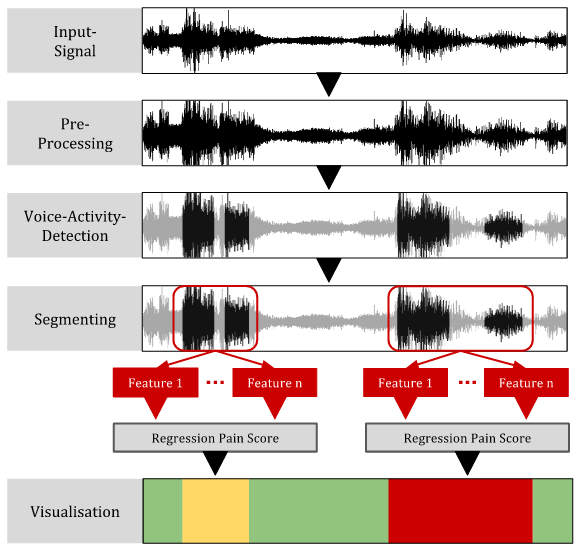
\includegraphics[width=0.75\textwidth]{bilder/pipeline01.png}
	\caption{Die Verarbeitungs-Pipeline des vorgestellten Systems}
	\label{img:architecture-overview}
\end{figure}

\section{Preprocessing}
\label{sec:preprocessing}

Beim Preprocessing wird das Signal so vorverarbeitet, dass Störeinflüsse auf die darauf folgenden Verarbeitungsschritte von vorneherein minimiert werden. Welches Pre-Processing durchgefüht wird, ist Abhägig von der konrketen Aufgabenstellung. So werden beispielsweise bei einigen Algorithmen zur Voice-Activity-Detection, also dem markieren stimmhafter Signalabschnitte, Tiefpass, Hochpass- und Bandpassfilter eingesetzt, um diejenigen Frequenzanteile herauszufiltern, die von der Stimme nicht produziert werden können \cite{vad_entropy} \cite{vad_ceps} \cite{vad_kola}. Bei einigen Pitch-Detection-Algorithmen wird \emph{Centerclipping} eingesetzt, also das 0-Setzen von Samples mit $ x[i] < 0.5 \cdot $ Maximalaussteuerung.\cite{czechPitch} 

In dieser Arbeit wurde sich für eine Vorverarbeitung entschieden, bei der das Signal hinsichtlich seiner Dynamik im Zeitbereich eingegrenzt wird. Dies ist ein typischer Vorverarbeitungschritt bei Sprachaufnahmen. Hintergrund ist, dass sehr kurz, aber sehr laute Pegelspitzen weit über dem Durchschnittspegel des Gesamtsignals den Maximalwert des Signals unnötig begrenzen und die Signalenergie so gering halten. Da die Testsignale, die in dieser Arbeit verwendet werden, aus inhomgenen Quellen stammen und sehr unterschiedliche Lautstärken haben, wird so gewährleistet, dass sie zumindest ähnliche Energien haben. An dieser Stelle werden (noch) keine Frequenanteile herausgefiltert, um keine Frequenzen zu verlieren, die in den späteren Verareitungsschritten wieder Voice-Activity-Detection \ref{sec:vad} oder der Feature-Extraction eventuell noch benötigt werden.

Die Dynamikeinschränkung wird mit Hilfe eines Audiokompressor umgesetzt. Ein Audiokompressor verringert Signalspitzen, die über einen festgelegten \emph{Schwellwert (Threshold)} liegen, um ein festgelegtes \emph{Verhältnis (Ratio)}. Ein Threshold von 0.3 mit Ratio von 0.5 bedeutet beispielsweise, dass alle Signalspitzen, die den Wert 0.3 überschreiten oder -0.3 unterschreiten, um 50\% verringert werden. Ein Kompressor kann auf die Überschreitung des Thresholds erst nach einer als \emph{Attack} bezeichneten Verzögerung reagieren, und bei erneuten Verlassen des Thresholdes mit einer als \emph{Release} bezeichneten Verzögerung nachwirken. Signalspitzen werden so verringert und die Lautstärke-Dynammik eingeschränkt. Die tatsächliche Erhöhung der Signalenergie geschieht im Anschluss durch die Anhebung der insgesamten Signallautstärke, wie Beispielsweise der Normalisierung des Signals auf den Maximalpegel. Abbildung \ref{img:compressor} zeigt die Parameter eines solchen Audio-Kompressors.

\begin{figure}[h]
	\centering
	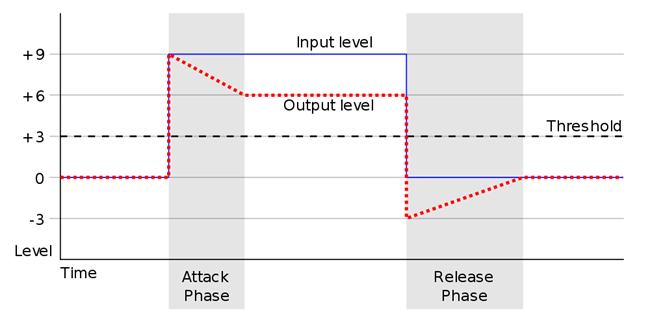
\includegraphics[width=0.6\textwidth]{bilder/compressor.png}
	\caption{Parameter eines Audio-Kompressors}
	\label{img:compressor}
\end{figure}

Der entwickelte Kompressor automatisiert die Einstellung von Threshold und Ratio auf Grundlage des Root-Mean-Square (RMS) des Signales $x$ der Länge $N$. Der RMS-Wert ist ein Maß für die durchschnittliche Signalenergie und wird wie nach Formel \ref{eq:rms} berechnet. Threshold und Ratio werden nach den Formeln \ref{eq:THold} und \ref{eq:ratio} berechnet, wobei der Parameter $r_a$ den Ziel-RMS-Wert anbgibt und mit dem Wert.

\begin{equation}
\text{RMS}(x) = \sqrt{\frac{1}{N}\sum_{n=0}^{N-1}x[n]^2}
\label{eq:rms}
\end{equation}
\begin{equation}
\text{THold}(x) = \bigg[\frac{\text{RMS}(x[])}{r_a}\bigg]^{2}
\label{eq:THold}
\end{equation}
\begin{equation}
\text{Ratio}(x) = \bigg[\frac{\text{RMS}(x[])}{r_a}\bigg]^{2}
\label{eq:ratio}
\end{equation}

Abbildung \ref{img:compressing01} zeigt das ein Signal vor und nach dem Preprocessings. Zu sehen ist, dass die Lautstärke der einzelnen Schrei-Einheiten nach der Anpassung einheitlicher ist. 

\begin{figure}[h]
	\centering
	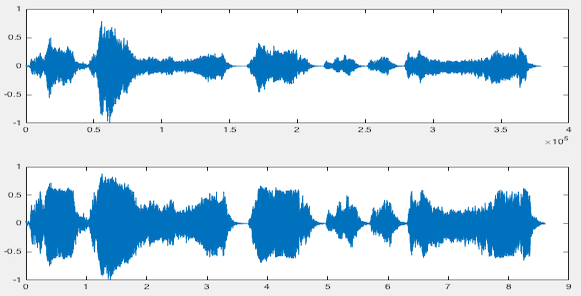
\includegraphics[width=0.6\textwidth]{bilder/compressing01.png}
	\caption{Ergebnis des Preprocessings}
	\label{img:compressing01}
\end{figure}

\section{Voice Activity Detection}
\label{sec:vad}

Das Ziel ist, in einem Audiosignal diejenigen Stellen zu markieren, in denen Stimme enthalten ist. Abbilung \ref{img:vad01} visualisiert ein Beispiel für eine solche Markierung: Zu sehen ist der Zeitbereich eines Audiosignales mit drei klar erkennbaren Cry-Units. Die rote Linie, die das Signal überspannt, bildet die Zeiteinheiten des Eingangssignales in die binären Kategorien \emph{Stimmhaft} und \emph{Stille} ab.

\begin{figure}
	\centering
	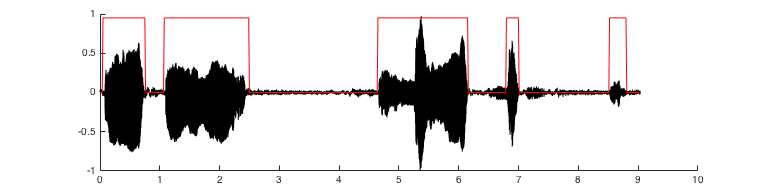
\includegraphics[width=0.7\textwidth]{bilder/vad_introduction01.png}
	\caption{Markierung von Schreigeräuschen im Audiosignal. Schwarz: Das Eingangssignal $x[\;]$. Rot: Klassifizierung in Stimmhaft/Stille}
	\label{img:vad01}
\end{figure}

Die Erkennung des Vorhandenseins von Stimme in einem Signal wird als \emph{Voice Activity Detection (VAD)} oder auch \emph{Speech Detection} bezeichnet. Das Ziel ist die Unterscheidung von denjenigen Zeiträumen im Signal, in denen Stimme enthalten ist, von den Zeiträumen ohne Stimme. Die größte Herausforderung für VAD-Algorithmen ist die robuste Erkennung bei Signalen mit Rauschen unbekannter Stärke und Natur. \cite[S. 1]{vad_kola} \cite[S. 1]{vad_Lisboa}

Der Grundlegende Aufbau eines VAD-Algorithmus ist wie folgt:
\begin{enumerate}
	\item \textbf{Windowing}: Unterteilung des Signals in (einander überlappende) Fenster, für die Entscheidung durchgeführt werden soll.
	\item \textbf{Feature-Extraction} aus den einzelnen Fenstern
	\item \textbf{Thresholding / Klassifizierung} über die Präsens oder Nicht-Präsens von Stimme für jedes Zeitfenster auf Grundlage der Extrahierten Features mit Hilfe von Entscheidungsregeln wie Grenzwerten.
	\item \textbf{Decision-Smoothing}, das nachträgliche Hinzufügen oder Entfernen von Entscheidungen mit Hilfe von kontextuellen Informationen der umliegenden Entschiedungen.\cite[S. 8 - 9]{vad_granada} \cite[S. 1 - 2]{vad_kola}
\end{enumerate}

Der an dieser Stelle entwickelte Ansatz ist eine Kombination aus den Ideen, die von  Moattar et al \cite{vad_Easy}, Kristjansson et al \cite{vad_Lisboa}, Waheed et al \cite{vad_entropy}, Ahmadi et al \cite{vad_ceps} und Shen et al\cite{vad_entropie02} vorgestellt wurden. 

\subsection{Windowing}
\label{sec:windowing}

Das Signal $x[\;]$ wird nach den in Kapitel \ref{sec:stft} beschriebenen Verfahren nach Gleichung \ref{eq:signal-Window} in die Signalfenster $x_0[\;] \ldots x_m[\;]$ zerlegt, bezeichnet als \glqq Windowing\grqq{}. Die Signalfenster werden zunächst im Zeitbereich belassen. Es wurde sich für die Waheed et al \cite{vad_entropy} vorgestellte Fensterlänge von \SI{25}{\milli\second} entschieden, als Kompromiss zwischen den von Moattar et al\cite{vad_Easy} empfohlenen \SI{10}{\milli\second} und den von Ahmadi et al \cite{vad_ceps} empfohlenen \SI{40}{\milli\second}. Die Fenster überlappen einander um 50\%, das heisst \SI{12.5}{\milli\second}.

\subsection{Feature Extraction}
\label{sec:featExtraction}

Für jedes Signalfenster $x_0[\;]...x_m[\;]$ à \SI{25}{\milli\second} werden die folgenden Features aus den Kategorien \textbf{Zeit-Bereich}, \textbf{Frequenz-Bereich}, \textbf{Cesptrum} und \textbf{Auto-Korrelation} berechnet.

\subsubsection{Zeit-Bereich}
\label{sec:timeFeats}

Im Zeit-Bereich werden die beiden Features \emph{Root-Mean-Square}-Wert \emph{[RMS]} und \emph{Zero-Crossing-Rate} \emph{[ZCR]} berechnet. 

Moattar et al \cite{vad_Easy} bezeichnen den Energiegehalt eines Signals als das für die VAD am häufigsten Angewandte Feature. Daher wird der RMS-Wert eines Signalfensters nach Gleichung \ref{eq:rms} verwendet. Hintergrund ist, dass der Energiegehalt eines Stimmsignals typischerweise Höher ist als der des Hintergrundrauschens. Bei geringen Signal-to-Noise-Ratios ist diese Bedingung jedoch nicht immer gegeben. Als zweites Feature des Zeitbereiches wird die in verwendete \emph{Zero-Crossing-Rate} berechnet. Die ZCR nach Formel \ref{eq:zcr} gibt an, wie häufig ein Vorzeichenwechsel im Signal vorkommt. Eine höhere ZCR weist auf Stille hin, da Rauschen typischerweise einen höheren ZCR als Signale mit einer Periodizität aufweist. Problematisch ist dieses Kriterium bei Signalen, bei denen gar kein Hintergrundrauschen vorliegt, da solche Signalfenster eine ZCR von 0 aufweisen. \cite{vad_ceps} 

\begin{equation}
\text{ZCR}(x_i[\;]) = \sum_{1}^{N-1}|\text{sng}(x_i[n])-\text{sng}(x_i[n-1])|
\label{eq:zcr}
\end{equation}

%Abbildung \ref{img:VAD_TDsignals} visualisiert diese beiden Features Anhand eines Beispielsignals Signal/Rausch-Abstand von \SI{20}{\decibel}. Es handelt sich um das selbe Signal wie aus Abbildung \ref{img:vad01}. Für jedes Signalfenster wurden der RMS-Wert und die ZCR berechnet. Die Features werden ebenfalls als Signal dargestellt, indem für den Anfangszeitpunkt eines Zeitfenster der jeweilige berechnete Feature-Wert abgetragen wird. Die Feature-Signale wurden so skaliert, dass ihr Maximalwert 1 nicht überschreitet, um ihr Verhalten bezüglich des Vorhandenseins von Stimme klarer erkennbar zu machen.

%\begin{figure}[h]
%	\centering
%	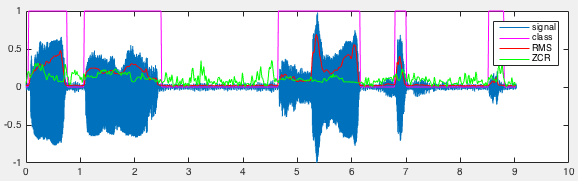
\includegraphics[width=0.6\textwidth]{bilder/VAD_TDsignals.png}
%	\caption{Features des Zeitbereiches}
%	\label{img:VAD_TDsignals}
%\end{figure}

\subsubsection{Autokorrelation}

Neben den in Kapitel \ref{sec:featExtraction} geannten \glqq einfachen\grqq{} Features des Zeitbereiches  wird zur VAD die Autokorrelation verwendet. Wie in Kapitel \ref{sec:theVoice} ausgeführt, weisen stimmhafte Signale eine höhere Periodizität als das Hintergrundrauschen auf. Daher eignet sich die in Kapitel \ref{sec:autocorrelation} vorgestellte Autokorrelation, um diese Periodizität festzustellen. Es werden die Features \emph{Maximum Autocorrelation Peak} [\emph{aMax}] und (\emph{Autocorrelation Peak Count}) [\emph{aCount}] berechnet. 

Beide Features werden von Kristjansson et al \cite[S. 1 - 2]{vad_Lisboa} zur VAD erprobt. Die \emph{höchste Magnitude der Autokorrelation }  (\emph{Maximum Autocorrelation Peak}) wird nach der Formel \ref{eq:corrpeak} definiert und bestimmt die höchste Magnitude im Autokorrelations-Signal. Eine höherer [\emph{aMax}]-Wert spricht für eine dominante Grundfrequenz im Signal. Das zweite Feature ist die \emph{Anzahl an Autokorrelations-Spitzen} nach Formel \ref{eq:corrcount}. Ein höherer [\emph{aCount}]-Wert spricht für das vorhandensein dominanter Obertonwellen im Signal. Aus Kapitel \ref{sec:acousticModel} geht hervor, dass die Grundfrequenz von Neugeborenen zwischen $200 - \SI{2000}{\hertz}$ liegt, weshalb auch nur in Lags dieses Bereichs die Autokorrelation durchgeführt wurde.

\begin{equation}
\text{aMax}(x_i[\;]) = \max_{k}\text{mag}\{\text{NA-Corr}_k(x_i[\;])\}
\label{eq:corrpeak}
\end{equation}

\begin{equation}
\text{aCount}(x_i[\;]) = \counti_{k}\text{mag}\{\text{NA-Corr}_k(x_i[\;])\}
\label{eq:corrcount}
\end{equation}

%Abbildung \ref{img:VAD_CoDsignals} visualisiert die Features der Autokorrelation auf die selbe Art und Weise wie bei Abbildung \ref{img:VAD_TDsignals}.

%\begin{figure}[h]
%	\centering
%	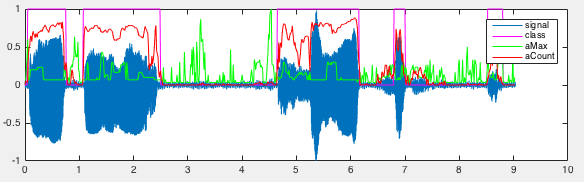
\includegraphics[width=0.6\textwidth]{bilder/VAD_CoDsignals.png}
%	\caption{Features der Autokorrelation}
%	\label{img:VAD_CoDsignals}
%\end{figure}

\subsubsection{Frequenz-Bereich}

Aus dem \textbf{Frequenz-Bereich} werden die drei Features \emph{unnormalisierte spektrale Entropie} $[SEnt_{u}]$, \emph{normalisierte spektrale Entropie}  $[SEnt_{n}]$ und \emph{dominanteste Frequenzkomponenten} $[f_{Dom}]$ berechnet. 

Als Vorbereitungsschritt werden die Signalfenster des Zeit-Bereiches $x_0[\;] \ldots x_m[\;]$ zunächst mit der in Kapitel \ref{sec:stft} vorgestellten Short Time Fourier Transformation in die \emph{Frequenz-Fenster} \label{eq:stft} $X_0[\;] \ldots X_m[\;]$ transformiert. Das heißt, dass $X_i[\;] = \text{DFT}(w[\;] \cdot x_i[\;])$. Es wurde eine $2048$ Punkte Lange FFT und eine Hamming-Window als Fensterfunktion verwendet.

Kristjansson et al \cite[S. 2]{vad_Lisboa} verwenden die \emph{spektrale Entropie} Voice Activity Detection. Dabei wird das Spektrum des Frequenzfensters $X_i$ als Wahrscheinlichkeitsverteilung betrachtet. Die Entropie als Maß zur \glqq Unreinheit\grqq{} wird in Kapitel \ref{sec:id3} erläutert. Die \emph{normalisierte spektrale Entropie} wird nach der Formel \ref{eq:norm_se} berechnet. Das Signal $px_i[\;]$ ergibt sich durch die Normalisierung des $N$-Punkte langen Spektrums nach Formel \ref{eq:norm_spek}. Neben der in \cite{vad_Lisboa} vorgestellten normalisierten spektralen Entropie wird zusätzlich die \emph{unnormalisierte Spektrale Entropie} nach Formel \ref{eq:unnnorm_se} berechnet. Bei dieser wird das Spektrum nicht normalisiert, das heißt, es gilt $px_i[f] = X_i[f]$. Somit hat Energie des Signals einen größeren Einfluss die höhe des Features. Bei der normalisierten spektralen Entropie ist zu erwarten, dass Frequenzfenster mit Hintergrundrauschen eine höhere Entropie haben als Fenster mit Stimme . Bei der unnormalisierten spektralen Entropie ist zu erwarten, dass Signalfenster mit Stimme eine höherer Spektrale Entropie haben als Fenster mit Stille.\footnote{Kristjansson et al \cite[S. 2]{vad_Lisboa} verwenden zur Entropie-Berechnung den Logarithmus zur Basis 10, anstatt zur Basis 2. Es ist nicht klar, ob es sich dabei um einen Fehler handelt. Zur Featureberechnung in dieser Arbeit wurde, wie in dem Paper beschrieben, ebenfalls der Logarithmus zur Basis 10 verwendet!}

In die Berechnungen wurden nur die Frequenzen im Bereich von 200 - \SI{8000}{\hertz} mit einbezogen, da aus Kapitel \ref{sec:cryModel} die tiefst Mögliche Frequenz kindlicher Lautäußerung bei \SI{200}{\hertz} liegt und nach Shen et al \cite{vad_entropie02} Stimme keine Informationen oberhalb von \SI{8000}{\hertz} übertragen.

\begin{equation}
px_i[n] = \frac{X_i[n]}{\sum_{k=1}^{N} X_i[k]}
\label{eq:norm_spek}
\end{equation}

\begin{equation}
\text{SEnt}_n(px_i[\;]) = -\sum_{k=1}^{N}px_i[k] \cdot\log(px_i[k])
\label{eq:norm_se}
\end{equation}

\begin{equation}
\text{SEnt}_u(X_i[\;]) = -\sum_{k=1}^{N}X_i[k] \cdot\log(X_i[k])
\label{eq:unnnorm_se}
\end{equation}

Moattar et al \cite[S. 2550]{vad_Easy} stellen die \emph{dominanteste Frequenzkomponente} zur Voice-Activity-Detection vor. Für jedes Frequenzfenster $X_i[\;]$ wird diejenige Frequenz nach Formel \ref{eq:domfreq} berechnet, welches die höchste Amplitude hat. Es wird dabei, im Gegensatz zur spektralen Entropie, der gesamte Frequenzraum betrachtet. Ein stimmhaftes Signal hat typischerweise eine höhere $f_{Dom}$ als ein nicht stimmloses Signal, bedingt durch die hohe Amplitude der Grundfrequenz.

\begin{equation}
f_{Dom}(X_i[\;]) = \argmax_k\{X_i[k]\}
\label{eq:domfreq}
\end{equation}

%Abbildung \ref{img:VAD_FDsignals} visualisiert diese Features für das selbe Eingangssignal aus \ref{img:VAD_TDsignals}. Die Features wurden wie bei Abbildung \ref{img:VAD_TDsignals} beschrieben für die Darstellung skaliert

%\begin{figure}[h]
%	\centering
%	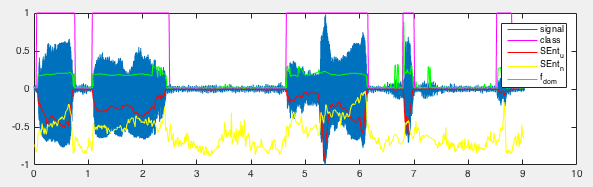
\includegraphics[width=0.6\textwidth]{bilder/VAD_FDsignals.png}
%	\caption{Features des Frequenz-Bereiches}
%	\label{img:VAD_FDsignals}
%\end{figure}

\subsubsection{Cepstrum}
\label{sec:cepstrum-feature}

In Kapitel \ref{sec:autocorrelation} wurde das Cepstrum vorgestellt und Erläutert, wie Peaks im oberen Quefrency-Bereich auf das Vorhandensein eines periodischen, obertonreichen Signals, wie die Stimme eines ist, hinweist. Aus dem Cepstrum-Bereich werden die Features \emph{Upper Cepstrum Peak} $[ Ceps_{mag} ]$ und \emph{Upper Cepstrum Peak Location} $[ Ceps_{loc} ]$ berechnet.

Ahmadi et al \cite{vad_ceps} sowie Kristjansson et al\cite{vad_Lisboa} schlagen vor, die \emph{höchste Magnitude im oberen Quefrency-Bereich} (Upper Cepstrum Peak) als Feature zu verwenden. Formel \ref{eq:ceps_maxpeak} definiert die Berechnung. $c_i[\;]$ ist das Cepstrum des $i$-ten Frequenzfenster $X_i[\;]$. Wie in Kapitel \ref{sec:acousticModel} erläutert, liegt die Grundfrequenz bei kindlichen Lautäußerungen zwischen 200 und \SI{2000}{\hertz}, was einem Quefrency-Bereich von 5 - \SI{40}{\milli\second} entspricht. Folglich werden bei der Berechnung nach Formel \ref{eq:ceps_maxpeak} nur Quefrency-Werte in diesem Bereich betrachtet. Eine hoher $Ceps_{mag}$-Wert weist auf das Vorhandensein von Stimme für das aus dem Fenster $x_i[\;]$ Berechneten Cepstrum $c_i[\;]$ hin. Als zweites Features wird die Quefrency der höchsten Amplitude des Cepstrum (Upper Cepstrum Peak Location) nach Formel \ref{eq:ceps_loc} berechnet. Bei Signalfenstern mit Stille ist es wahrscheinlicher, dass sich die höchste Ampltiude am Mindest- oder Maximum-Wert des durchsuchten Quefrency-Bereiches befindet.

\begin{equation}
Ceps_{mag}(c_i) = \max_{k}\text{mag}\{c[k]\}
\label{eq:ceps_maxpeak}
\end{equation}

\begin{equation}
Ceps_{loc}(c_i) = \argmax_{k}\{c[k]\}
\label{eq:ceps_loc}
\end{equation}


Abbildung \ref{img:vadAllFeatures} visualisiert alle vorgestellten Features, die für die Voice Activity Detection eingesetzt werden. Der oberste Plot zeigt das Audiosignal aus Abbildung \ref{img:vad01} mit einem Signal/Rauschabstand von \SI{20}{\decibel}. Der rote Graph über den Plot klassifiziert die Zeitbereiche in $1 = $ \emph{stimmhaft} und $0 = $ \emph{nicht stimmhaft}. Alle darunter eingezeichneten Plots zeigen den zeitlichen Verlauf der entsprechenden Features. Bei jedem Feature ist eine Korrelation mit der stimmhaftigkeit oder nicht-stimmhaftigkeit der entsprechenen Signalabschnitte zu sehen, welche bei einigen Feature stärker ausfällt als bei anderen..

\begin{figure}[h!]
	\centering
	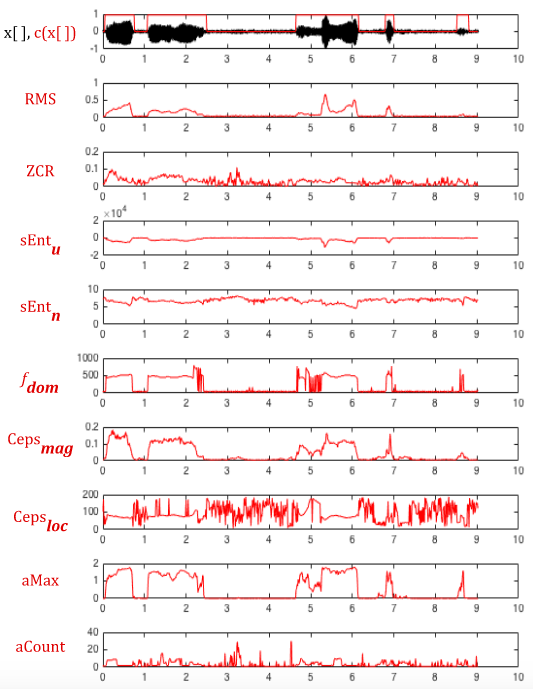
\includegraphics[width=0.8\textwidth]{bilder/allFeatures01.png}
	\caption{Übersicht über alle Features, die für die Voice Activity Detection verwendet werden.}
	\label{img:vadAllFeatures}
\end{figure}

\subsubsection{Konstruktion des Feature-Raumes}

Abbildung \ref{img:min-signal} zeigt in (A) des zeitlichen Verlauf des \emph{RMS}-Features eines Signals mit einem Signal-Rausch-Abstand (SNR) von \SI{50}{\decibel}. Die Zeiträume mit Stille haben einen weitaus niedrigeren RMS-Wert als die Zeiträume mit Stimme. In (B) ist das selbe Signal mit einem Signal-Rausch-Abstand von \SI{3}{\decibel} zu sehen. Nun liegen die RMS-Werte der stimmlosen Bereiche nur noch knapp unter denen des Sprachsignals. Zu sehen ist, dass starkes Hintergrundrauschen ähnlich hohe Feature-Werte erzeugen kann wie die Stimme.

\begin{figure}[h]
	\centering
	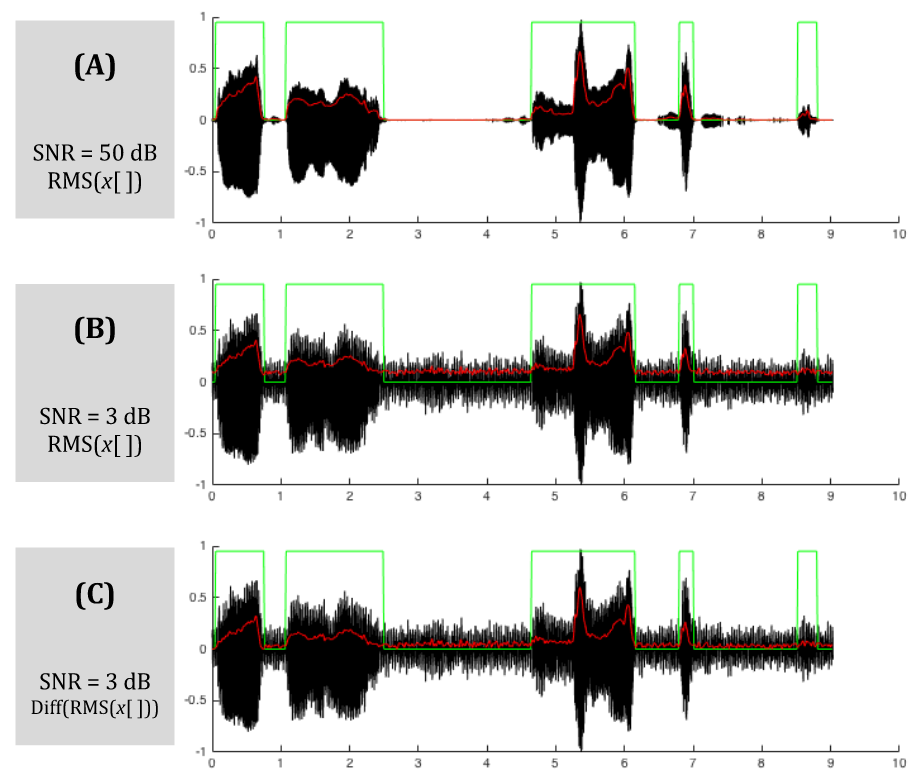
\includegraphics[width=0.7\textwidth]{bilder/rms_diff.png}
	\caption{Das RMS-Feature bei verschiedenen Signal/Rausch-Abständen. Schwarz: Eingangs-Signal $x[\;]$. Grün: Klassifizierung in Stimmhaft/Stille. Rot: Feature-Wert.}
	\label{img:min-signal}
\end{figure}

Moattar et al \cite{vad_Easy} und Waheed et al \cite{vad_entropy} präsentieren die Idee, den Wert des jeweiligen Features zu messen, der in den stimmlosen Bereichen durch das Hintergrundrauschen erzeugt wird. So kann davon ausgegangen werden, dass die ersten Signalfenster zunächst noch keine Stimme enthalten, und der Feature-Wert des Rauschens somit anhand der ersten Signalfenster bestimmt werden. Bei einer langanhaltenden und kontinuierlichen Analyse können sich die Signal/Rausch-Verhältnisse jedoch ständig ändern, weshalb der Feature-Werte der stimmlosen Signalbereiche regelmäßig aktualisiert werden müssem. Es kann jedoch davon ausgegangen werden, dass die Länge einer Cry-Unit eine bestimmte Länge $t_{max}$ nicht überschreiten kann, bevor das Babie Luft holen muss und somit ein Zeitfenster mit Stille entsteht. So haben Zeskind et al \cite{rythmic} diesen Wert mit $t_{max} = \SI{4.75}{\second}$ festgstellt. In einem Zeitbereich $ t > t_{max}$ muss somit zumindest ein Feature-Wert enthalten sein, der durch stimmlose Signalteile erzeugt wird. Auf Basis dieser Überlegung wird das \emph{Differenz-Feature} Diff($Feat(x_i[\;])$) nach Formel \ref{eq:difFeature} definiert als die Differenz des aktuell gemessenen Feature-Wertes und des geringsten Feature-Wertes, welcher im vergangenen Zeitbereich $t$ gemessen wurde. $Feat(x_i[\;])$ ist dabei ein beliebiger Feature-Wert des Signalfensters $x_i[\;]$, $t_{xi}$ die Länge eines Signalfensters in Sekunden $x_i$ ist (in diesem Fall \SI{25}{\milli\second}), und $t$ der in der Vergangenheit zu durchsuchende Zeitbereich in Sekunden, welcher größer als $t_{max}$ gewählt wird. In Abbildung \ref{img:min-signal} wird in (C) das Differenz-Feature für den RMS-Wert gezeigt.

\begin{equation}
\text{Diff}_t(Feat(x_i[\;])) = Feat(x_i[\;])\ - \mini_{k=i-z...i}( Feat(x_k[\;])), \qquad z = \frac{2 t}{t_{xi}}
\label{eq:difFeature}
\end{equation}

Der Feature-Raum setzt sich schlussendlich folgendermaßen zusammen: Die ersten 9 Features bilden die in Kapitel \ref{sec:timeFeats} - \ref{sec:cepstrum-feature} insgesamt 9 vorgestellten Features \emph{RMS, ZCR, SEnt\textsubscript{u}, SEnt\textsubscript{n}, $f_{Dom}$, Ceps\textsubscript{mag}, Ceps\textsubscript{loc}, aMax} und \emph{aCount}. Weiterhin wird für jedes Feature nach Formel \ref{eq:difFeature} das Differenz-Feature mit $t = \SI{5}{\second}$  berechnet. Die Features \emph{ZCR, SEnt\textsubscript{u}} und \emph{aCount} wurden vor der Berechnung des Differenz-Features bezüglich ihres Vorzeichens invertiert, da bei Ihnen ein hoher anstatt ein niedriger Wert stimmhafte Signalteile anzeigt. Das einzige Feature, welches nicht als Differenzfeature dem Feautrevektor beigefügt wurde, ist der \emph{Upper Cepstral Peak Location}-Feature [$Ceps_{loc}$], da es bei Stille sowohl einen höheren als auch einen niedrigeren Wert annehmen kann. Der Feature-Raum umfasst somit insgesamt $9 + 8 = 17 $ Dimensionen. Gleichung \ref{eq:featureVektor} verdeutlicht die Zusammensetzung des Feature-Vektors $v_i$, der aus dem Signalfenster $x_[\;]$ berechnet wird.

\begin{equation}
v_i = \Big( \text{RMS}(x_i[\;]), ...,\text{ aCount}(x_i[\;]), 
\text{Diff}_{t}(\text{RMS}(x_i[\;])) .... \text{Diff}_{t}(-\text{ aCount}(x_i[\;]))\Big)
\label{eq:featureVektor}
\end{equation}

\subsection{Thresholding}

\subsubsection{Finden der Grenzwerte}

Wird die Voice-Activity-Detection für ein Signal $x[\;]$ durchgeführt, wird es in die Signalfenster $x_1[\;]...x_n[\;]$ zerlegt  die Featurevektoren $v_1...v_n$ berechnet. Das Ziel ist nun, Grenzwerte für die Features zu finden, bei deren Über- oder Unterschreitung das Signalfenster als \emph{stimmhaft} kategorisiert wird. Abbildung \ref{img:thresholded} verdeutlicht das Prinzip für das Feature \emph{RMS}. Diese Entscheidung nach einem Grenzwert ist ein klassisches Vorgehen bei der Voice-Activity-Detection. Eine binäre Klassifizierung nach dem Muster $C(x_i) = \{ 1, \text{wenn } \text{RMS}(x_i[\;]) \geq 0.18 ,\quad 0 \text{ sonst}\}$ würde auf den in diesem Fall für eine weitgehend richtige Klassifizierung vornehmen.

\begin{figure}[h]
	\centering
	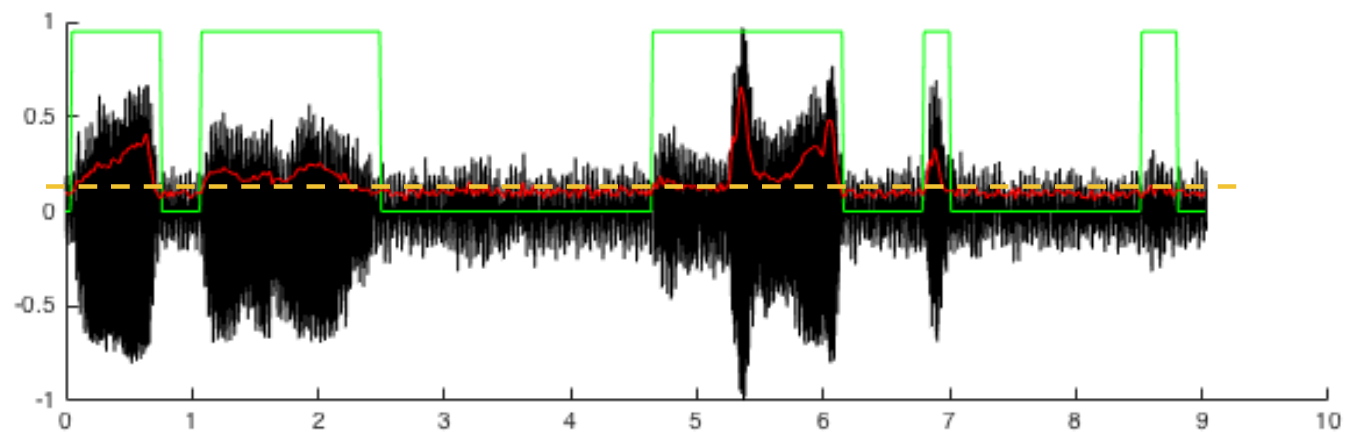
\includegraphics[width=0.6\textwidth]{bilder/thresholded02.png}
	\caption{Thresholding eines Feature-Signales. Schwarz: Das Signal $x[\;]$. Grün: Klassifizierung in Stimmhaft/Stille. Rot: RMS-Feature. Orange: Beispiel-Grenzwert}
	\label{img:thresholded}
\end{figure}

Eine Methode zum Finden der optimalen Grenzwerte ist der in Kapitel \ref{sec:c45} vorgestellte \emph{C4.5}-Algorithmus. Da der \emph{C4.5} Entscheidungsbäume erstellt, kann die Entschiedung aufgrund der Verkettung von Grenzwerten mehrerer Features gefällt werden. Ein Beispiel wird in Listing \ref{lst:tree01} dargestellt, bei dem die Klasse eines  Signalfensters hierarchisch zuerst nach einem Grenzwert für Ceps$_{mag}$ und danach für den RMS-Wert entschieden wird.

\begin{lstlisting}[frame=single,mathescape=true,basicstyle=\footnotesize,language=Java,label=lst:tree01,caption=Beispiel eines CART-Entscheidungsbaums,linewidth=1\textwidth]
if Ceps$_{mag}$($x_i[\;]$) > 0.2
|   if RMS($x_i[\;]$) < 0.13
|   |   C($x_i[\;]$) = 0
|   |else
|   |   C($x_i[\;]$) = 1
|else
|    C($x_i[\;]$) = 1
\end{lstlisting}

\subsubsection{Trainings- und Testdatensätze}
\label{sec:databases}

Zur Training und zur Evaluation des REPTree muss ein Datensatz $D$ erstellt werden, dessen Erzeugung in diesem Kapitel beschriebn wird. 

Es wurden sechs Audioaufnahmen mit Weinen von Babies von der freien Online-Sound-Bibliothek \url{https://www.freesound.org/} heruntergeladen und zu Segmenten à 10 Sekunden beschnitten. Es handelt sich um weitgesgehend rauschfreie Aufnahmen, die von verschiedenen Babys stammen. In den Audiosignalen wurden manuell die Zeitbereiche markiert, welche Stimme enthalten. Es wurden \emph{keine} Geräusche markiert, bei denen es sich offensichtlich um Einatumungs-Geräusche handelt. Geräusche, bei denen nur Anhand der Aufnahme nicht mit Sicherheit festgestellt werden konnte, es ob sie durch Einatmungs- oder Ausatmungs-Geräusche handelt, wurden als Stimme markiert. Weiterhin wurden drei verschiedene Rauschsignale heruntergeladen. Es handelt sich um \glqq realistische\grqq{} Atmosphären von Krankenhäusern. Jedes der sechs Audioaufnahmen der Babys wurde mit jedem der drei Rauschsignale überlagert, einmal mit einem Signal/Rausch-Abstand von \SI{50}{\decibel} (\glqq fast unhörbares Rauschen\grqq), und einmal mit einem Signal/Rausch-Abstand von \SI{3}{\decibel} (\glqq starkes Rauschen\grqq). Außerdem wurde ein siebte Aufnahme eines Babies heruntergeladen, welches mit einem vierten Rauschsignale mit einem SNR von \SI{7}{\decibel} überlagert wurde. Dieses Signal spielt eine Sonderrolle, da es bei der Konstruktion der Entscheidungsbäume nur zur Verifikation verwendet wird. So wurden vier Mengen an Audiosignalen erzeugt:

\begin{description}
	\item[A\textsubscript{\SI{50}{\decibel}}] enthält $3 \cdot 6=18$ Audiosignale, bei dem alle sechs Baby-Aufnahmen mit den drei Rauschsignalen bei einem Signal-Rausch-Abstand von \textbf{\SI{50}{\decibel}} überlagert wurden
	
	\item[A\textsubscript{\SI{3}{\decibel}}] enthält $3 \cdot 6=18$ Audiosignale, bei dem alle sechs Baby-Aufnahmen mit den drei Rauschsignalen bei einem Signal-Rausch-Abstand von \textbf{\SI{3}{\decibel}} überlagert wurden
	
	\item[A\textsubscript{50+\SI{3}{\decibel}}] $ = \{ A_{\SI{50}{\decibel}} \cup  A_{\SI{3}{\decibel}}\} = 32$ Audiosignale
	
	\item[A\textsubscript{\SI{7}{\decibel}*}] enthält $1$ Audiosignal, bei dem eine siebte Baby-Aunfahme mit einem vierten Rauschsignal bei einem Signal-Rausch-Abstand von \textbf{\SI{7}{\decibel}} überlagert wurde.
	
\end{description}

Im nächsten Schritt werden die eigentlichen Datensätze $D_{SNR,Feats}$ gebildet, in dem Audiosignale dieser Signalmengen (1) wie in Kapitel \ref{sec:preprocessing} beschrieben vorverarbeitet werden, (2) wie in Kapitel \ref{sec:windowing} in die Signalfenster à \SI{25}{\milli\second} zerlegt werden und (3) für jedes Signalfenster der durch Gleichung \ref{eq:featureVektor} definierte Featurevektoren berechnet wird. Außerdem wird jedem Featurevektor die Klasseninformation \emph{Stimme/Stille} zugewiesen.

Es ist rechnerisch zu aufwendig, alle genannten Features in einem kontinuierlichen System zur Voice Activity Detection zu berechnen. Daher werden die Datensätze in Untermengen bezüglich der verwendeten Features eingeteilt. Das Ziel ist es, diejenige Untermenge an Features zu finden, die sich am besten für die Voice-Activity-Detection sowohl bei niedrigem als auch bei starkem Hintergrundrauschen eignet. Die Untermengen werden in Bezug auf die Methode gebildet, durch die die Features berechnet werden. Das heißt, dass beispielsweise die Untermenge \emph{Zeit} die in Kapitel \ref{sec:timeFeats} beschriebenen Features \emph{RMS} und \emph{ZCR} sowie die dazugehören Differenzfeatures \emph{Diff\textsubscript{t}(RMS)} und \emph{Diff\textsubscript{t}(ZCR)} beinhaltet. 

Die 9 Untermengen sind: \{ Zeitbereich, Frequenzbereich, Cepstrum, Autokorrelation, Zeit + Frequenzbereich, Zeit + Cepstrum, Zeit + Autokorrelation, Frequenz + Cepstrum, Frequenz + Autokorrelation \}. Cepstrum- und Autokorrelation werden nicht gemeinsam in eine Untermenge hinzugefügt, da Sie die Rechnerisch aufwendigsten sind. So enthält beispielsweise der Datensatz $D_{\SI{3}{\decibel},Zeit}$ die Featurevektoren des Zeitbereiches für die Audiosignale mit einem Signal-Rausch-Abstand von \SI{3}{\decibel}. Alle Audiosignal-Mengen [A\textsubscript{\SI{50}{\decibel}}], [A\textsubscript{\SI{3}{\decibel}}], [A\textsubscript{50+\SI{3}{\decibel}}] und [A\textsubscript{\SI{7}{\decibel}}] wurden in Datensätze umgewandelt. Es wurden schlussendlich $4 \cdot 9 = 36$ Datensätze gebildet.

\subsubsection{Training} 
\label{sec:training}

Das Ziel ist, mit Hilfe des C4.5-Algorithmus einen Entschidungsbaum zu finden, der auf Basis einer möglichst geringen Feature-Menge eine möglichst hohe Klassifkationsgenauigkeit für sowohl niedrige als auch hohe Signal/Rausch-Abstänge erzielt. Die Frage ist, ob ein Entschiedungsbaum, der auf Basis von Signalen mit einem niedrigen SNR gebildet wird, auch für hohe SNR eine hohe Klassifikationsgenauigkeiten erzielt, oder ob der umgedrehte Fall zutreffend ist. Daher werden die Entscheidungsbäume sowohl auf Basis verschiedener SNRs als auch verschiedener Feature-Untermengen gebildet. Die Entschäudungsbäume werden daraufhin gegen die Signale mit den verschiedenen SNRs evaluiert. Wird also beispielsweise der Datensatz $D_{\SI{50}{\decibel},Zeit}$ zum Training und der Datensatz $D_{\SI{3}{\decibel}}$ verwendet, so wird berechnet, wie gut sich der Klassifikator unter Verwendung der Zeit-Features zur Klassifizierung niedriger SNRs eignet, obwohl er für hohe SNRs entworfen wurde. Dabei ist unerheblich, welche Features der Test-Datensatz verwendet, da es bei der Evaluation nur auf die Klasseninformation der Instanzen ankommt.

Die Implementierung, die für den \emph{C4.5} verwendet wurde, ist der \emph{REPTree}-Algorithmus \footnote{Dokumentation von REPTree: \url{http://weka.sourceforge.net/doc.dev/weka/classifiers/trees/REPTree.html}} der Open Source Data-Mining-Bibliothek \emph{Weka}\footnote{Download von WEKA: \url{http://www.cs.waikato.ac.nz/ml/weka/}}. Die Implementierung hat den Vorteil, dass die maximale Tiefe des Entscheidungsbaumes festlegbar ist und somit die Komplexität des Baumes begrenzt werden kann und Overfitting vermieden wird.

Es wurden insgesamt $3 \cdot 9 = 27$ Trainings-Datensätze erzeugt ( [3 SNR-Werte: \SI{3}{\decibel}, \SI{50}{\decibel} und 50+\SI{3}{\decibel} ] $\times$ [9 Feature-Untermengen]. Der Datensatz mit einem SNR von \SI{7}{\decibel} wurde \emph{nicht} zum Training verwendet). Mit diesen 27 Trainingsdatensätze wurden mit Hilfe des \emph{REPTree}-Algorithmus 27 Klassifikationsbäume erzeugt. Jeder Klassifikationsbaum wurde gegen die 3 Testdatensätze D\textsubscript{\SI{3}{\decibel}}, D\textsubscript{\SI{50}{\decibel}} und D\textsubscript{\SI{7}{\decibel}*} evaluiert und die Accuracy berechnet. Das Signal A\textsubscript{\SI{7}{\decibel}*} erfüllt dabei eine Sonderrolle, da es nicht in den Trainingsdatenstäzen enthalten war und somit der Kontrolle dient, ob Overfitting vorliegt. Da jeder Datensatz ungefähr dreimal mehr Stimmhafte Examples als nicht-Stimmhafte enhthielt, wurde jede Stimmlose Instanz eines Datensatzes eingefügt. Somit wurde für jeden Datensatz  ein ausgewogenes Verhältnis zwischen positiven und negativen Examples gewährleistet. Um die Komplexitiät des Entscheidungsbaumes zu verringern eine Nutzung von möglichst wenig Features zur Klassifizierung zu erzwingen, wurde die maximale Tiefe des REPTree auf 2 gesetzt. 

\subsubsection{Ergebnis} 
\label{sec:vad_result}

Die Evaluations-Ergebnisse  sind in Tabelle \ref{tab:reptree_results} zu sehen. Für jeden Trainingsdatensatz mit einem bestimmten SNR und einer Feature-Untermenge wird die Accuracy für den jeweilgen Test-Datensatz mit einem SNR von \SI{3}{\decibel}, \SI{50}{\decibel} und \SI{7}{\decibel}* verwendet.\footnote{Der Stern verdeutlicht die Sonderrolle des  Datensatzes mit einem SNR von \SI{7}{\decibel}, da er nur zu Evaluation verwendet wurde }. Außerdem wird der Durchschnittswert aller drei Accuracy-Werte angegeben.

Die Features, welche zu den höchsten Accuracy-Werten führten, sind die des \emph{Cepstrum}-Bereiches, genauer gesagt das Diff\textsubscript{t}(Ceps\textsubscript{mag})-Feature, da es vom REPTree als einziges Feature dieses Bereiches für die Entscheidungsbäume ausgewählt wurde. Die Entscheidungsbäume, die mit dem Diff\textsubscript{t}(Ceps\textsubscript{mag})-Feature entworfen wurden, erreichten eine durchschnittliche Accuracy von mindestens 91,45\%. Der nächstbeste Entscheidungsbaum mit einer Accuracy von 86,96\% wurde unter Verwendung der Features des Zeitbereiches und der Autokorrelation auf dem Datensatz D\textsubscript{50+\SI{3}{\decibel},Zeit+Correlation} entworfen. Sobald der Cepstrum-Bereich in Verbindung mit den Features anderer Bereiche verwendet wurde, wurde das Diff\textsubscript{t}(Ceps\textsubscript{mag})-Feature vom REPTree-Algorithmus bevorzugt und die Features der anderen Bereiche nicht mehr verwendet.

Auf Basis der Datensätze D\textsubscript{\SI{3}{\decibel},Ceps}, D\textsubscript{\SI{3}{\decibel},Zeit+Ceps}, D\textsubscript{\SI{3}{\decibel},Freq+Ceps}, D\textsubscript{50+\SI{3}{\decibel},Ceps}, D\textsubscript{50+\SI{3}{\decibel},Zeit+Ceps} sowie D\textsubscript{50+\SI{3}{\decibel},Freq+Ceps} wurde der selbe Klassifikator erzeugt, der in Gleichung \ref{eq:cepTree01} zu definiert wird. Wie zu sehen ist, handelt es sich um einen einfachen Grenzwert des \emph{v.Diff\textsubscript{t}(Ceps\textsubscript{mag})}-Features, da trotz der höchst möglichen Baumtiefe von 2 nur eine Tiefe von 1 genutzt wurde.

\begin{equation}
C(v_i) = \begin{cases}
1, \quad \text{if } v.Diff_t(Ceps_{mag}) > 0.02, \\
0 \quad \text{else}
\end{cases}
\label{eq:cepTree01}
\end{equation}


Auf Basis der Datensätze D\textsubscript{\SI{50}{\decibel},Ceps} und D\textsubscript{\SI{50}{\decibel},Zeit+Ceps} wurde der Klassifikator nach Gleichung \ref{eq:cepTree02} erzeugt. Er unterscheidet sich von dem Klassifikator aus Gleichung \ref{eq:cepTree01} nur durch den Grenzwert.

\begin{equation}
C(v_i) = \begin{cases}
1, \quad \text{if } v.Diff_t(Ceps_{mag}) > 0.03, \\
0 \quad \text{else}
\end{cases}
\label{eq:cepTree02}
\end{equation}

Da der Klassifikator aus Gleichung \ref{eq:cepTree01} eine durchschnittliche Accuracy von 92,22\% und der Klassifikator aus Gleichung \ref{eq:cepTree02} eine unwesentlich geringere Accuracy von 91,45\% erzielt, wurden für beide Modelle die Specificity und Sensitivity berechnet, um eine Entscheidung für eines der beiden Modelle fällen zu können. Dazu wurden die Signalmengen A\textsubscript{\SI{3}{\decibel}}, A\textsubscript{\SI{50}{\decibel}} und A\textsubscript{\SI{7}{\decibel}*} in Frames à 100 Windows zerlegt und für jedes Zeitfenster die Senstivity, Specificity und Accuracy bezüglich der beiden Klassifikatoren berechnet. Die Ergebnisse werden als Boxplots in Abbildung \ref{img:boxplots} dargestellt. Die Modelle unterscheiden sich am stärksten bezüglich der Datensätze mit \SI{3}{\decibel} und \SI{7}{\decibel}. Der Klassifikator mit dem Grenzwert von 0.03 erzielt in beiden Fällen eine höhere Specificity, aber geringere Senstivitiy als das Modell mit dem Grenzwert bei 0.02. Es wurde sich für das Modell für mit einem Grenzwert von 0.02 entschieden, da durch die höhere Senstivity mehr Cry-Units erkannt werden, die in späteren Verarbeitungsschritten immernoch als False-Positives erkannt und verworfen werden können. Einmal im Prozess der VAD als Stimmlos markierte Fenster werden jedoch nicht weiter verarbeitet und gehen somit \glqq verloren\grqq. 

Der Finale Klassifikations-Funktion eines Signalfensters $C(x_i[\;])$ in $0 \longmapsto Stille$ oder $1 \longmapsto Stimme$ ist somit durch Gleichung \ref{eq:vad-final} gegeben, wobei $c_i[\;]$ das Cepstrum des Signalfensters ist.

\begin{equation}
C(x_i[\;]) = \begin{cases}
1, \quad \text{if } v.Diff_t(Ceps_{mag}(c_i[\;])) > 0.02, \\
0 \quad \text{else}
\end{cases}
\label{eq:vad-final}
\end{equation}

\subsection{Markierung der Cry-Units}
\label{sec:CryUnit}

Wird die Voice-Activity-Detection für das Signal $x[\;]$ nach Gleichung \ref{eq:vad-final} durchgeführt, ist das Ergebnis eine Zuordnung der Signalfenster $x_1[\;] \ldots x_n[\;]$ zu den Klassen $C(x_i[\;]) = 1$ \emph{Stimme} oder  $C(x_i[\;]) = 0$ \emph{Stille}. Varallyay \cite[S. 16 - 17]{cry_thesis} stellt die Idee vor, auf Grundlage der Informationen der Voice-Activity-Detection die Cry-Units zu extrahieren (welche er in seiner Publikation als Cry-Segmente beschreibt). Das genaue vorgehen konnte jedoch nicht eingesehen werden, da der Autor dieser Arbeit keine Zugriffsrechte auf die Publikation erhielt.

Waheed et al \cite{vad_entropy} stellen die Idee vor, zusammenhängende und ununterbrochene Ketten als \emph{stimmhaft} klassifizierter Signalfenster zu \emph{Stimm-Segmenten} zusammenzufassen. Dieser Ansatz wird übernommen, wobei ein Stimmsegment in dem Kontext dieser Arbeit einer \emph{Cry-Units} entspricht. Möglicherweise ist dies der Ansatz, den auch  Varallyay \cite[S. 16 - 17]{cry_thesis} gewählt hat. Abbildung \ref{img:cryUnit} veranschaulicht diese Gruppierung. 

\begin{figure}[h]
	\centering
	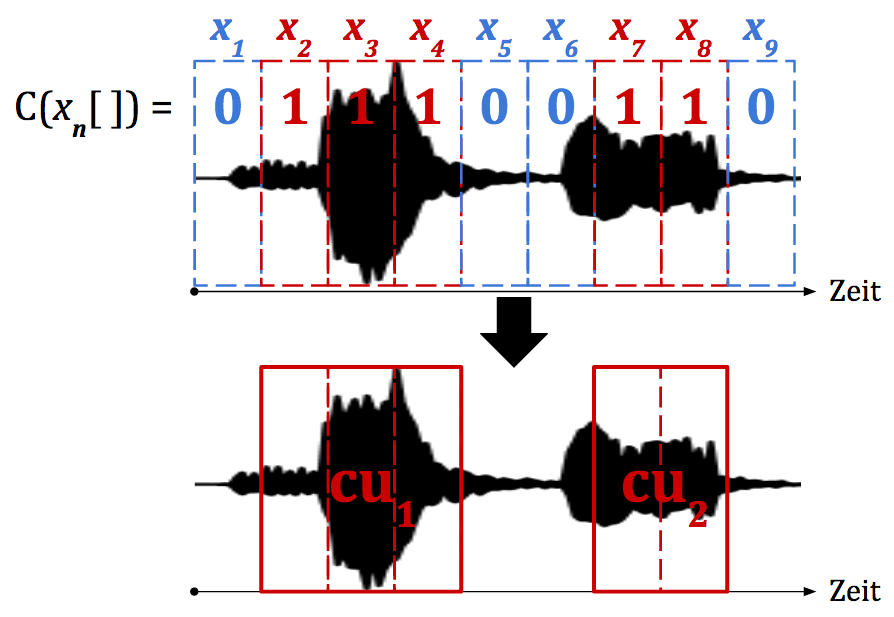
\includegraphics[width=0.6\textwidth]{bilder/cry-Unit02.png}
	\caption{Zusammenfassung klassifizierter Signalfenster zu Cry-Units}
	\label{img:cryUnit}
\end{figure}

Formel \ref{eq:cry-Unit} gibt die Definition des Datentypes \emph{Cry-Unit} $[CU]$. Eine Cry-Unit wird definiert durch den Anfangszeitpunkt $start$, einen Endzeitpunkt $end$ und der Liste seiner Signalfenster $windows = [x_1 ... x_m]$.

\begin{equation}
CU = (windows = [x_1 ... x_m ], start \in Zeit, end \in Zeit)
\label{eq:cry-Unit}
\end{equation}

Die Dauer eine Cry-Unit $cu \in CU$ wird nach Formel \ref{eq:cry-Lambda} berechnet und mit $\lambda$ bezeichnet. Der (Stille)-Zeitraum zwischen zwei Cry-Units d($cu_i, cu_j$), wird nach Formel \ref{eq:cry-distance} berechnet. Diese Zusammenhänge werden in Abbildung \ref{img:cryUnit-details} visualisiert.\cite{vad_entropy}

\begin{equation}
\lambda (cu) = cu.end - cu.start
\label{eq:cry-Lambda}
\end{equation}

\begin{equation}
\text{d}(cu_i, cu_j) = cu_j.start - cu_i.end
\label{eq:cry-distance}
\end{equation}

\begin{figure}[h]
	\centering
	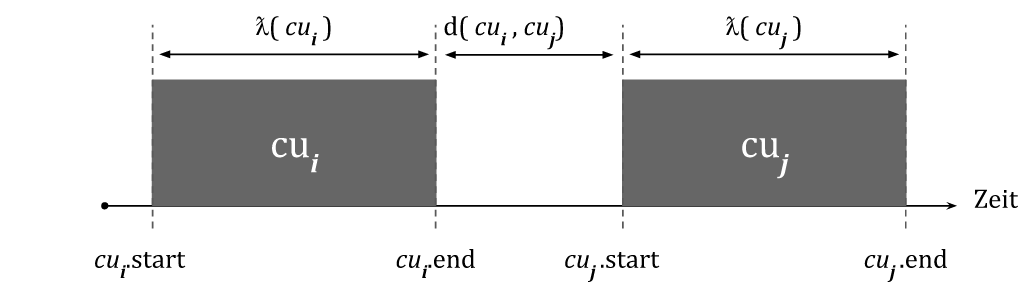
\includegraphics[width=0.8\textwidth]{bilder/newSmoothing05.png}
	\caption{Beziehung zwischen agrenzenden Cry-Units}
	\label{img:cryUnit-details}
\end{figure}

Algorithmus \ref{alg:cryUnit} zeigt in Pseudo-Code, wie auf Basis der Liste aller Signalfenster eines Signals $X_{all} = [x_1[\;] ,\ldots, x_n[\;]]$ die Liste der Cry-Units $CU_{all} = [cu_1 ... cu_m]$ generiert wird. Die Funktion $C(x)$ ist die Klassifikations-Funktion der Signalfenster in Stille/Stimme nach Gleichung \ref{eq:vad-final}. Die Funktion getTimeOf$(x_i[\;])$ liefert die Anfangszeitpunkt des Signalfensters $x_i[\;]$.

\begin{algorithm}[h]
	\caption{Gruppierung von Signalfenstern zu Cry-Units}
	\label{alg:cryUnit}
	\begin{algorithmic}[1]
		\Function{turnWindowsIntoCryUnits}{$X_{all}$}
		\State $ CU_{all} \gets [\;]$
		\State $ cu\gets ([\;],0,0)$
		\For{ $i = 1,\ldots,length(X_{all})$}
				\State $ c_i \gets C(x_i[\;])$
				\State \Comment Start of Cry-Unit
				\If {$c_i == 1 \wedge \text{isEmpty}(cu_j.windows)$}
						\State $ cu\gets ([\;],0,0)$
						\State $cu.start \gets \text{getTimeOf}(x_i[\;])$
						\State $cu.windows \gets [cu.windows, x_i[\;]]$
				\EndIf
				\State \Comment Inside Cry-Unit
				\If {$c_i == 1 \wedge \text{ ! isEmpty}(cu.windows)$}
						\State $cu.windows \gets [cu.windows, x_i[\;]]$
				\EndIf
				\State \Comment End of Cry-Unit
				\If {$c_i == 0 \wedge \text{ ! isEmpty}(cu.windows)$}
						\State $cu.end \gets  getTimeOf(x_i[\;])$
						\State $CU \gets [CU, cu]$
						\State $cu.windows \gets [\;]$
				\EndIf
		\EndFor
		
		\State \Comment End last Cry-Unit by force if is still open.
		\If {$\text{ ! isEmpty}(cu.windows) == 0$}
		\State $cu.end \gets  getTimeOf(X_{windows}[end])$
		\State $CU_{all} \gets [CU_{all}, cu]$
		\EndIf
		
		\Return $CU_{all}$
		
		\EndFunction
		
	\end{algorithmic}
\end{algorithm}

\subsection{Decision Smoothing}

Abbildung \ref{img:beforeSmoothing} zeigt ein Audiosignal mit einem Signal-Rausch-Abstand von \SI{3}{\decibel}, bei dem die Klassifikation nach Gleichung \ref{eq:vad-final} durchgeführt wurde. Die rote Linie zeigt die tatsächliche Klassifizierung und die grüne Linie die prognostizierte Klassifizierung. Die tatsächlichen/gefunden Cry-Units sind klar zu erkennen als die Bereiche, die von der roten/grünen Linie überspannt werden. Es ist zu sehen, dass False-Negatives und False-Positives in der Klassifizierung enthalten sind. Im folgenden werden drei charakteristische Arten falscher Klassifikationen näher erläutert:

\begin{description}
	\item [False Negatives nach (a) :] Eine korrekt erkannte, längere Cry-Unit wird zu früh beendet. Oft werden kurz nach dem Ende sehr kurze Cry-Units erkannt, die eigentlich noch zu der längeren, vorhergehenden Cry-Unit gehören.
	\item [False Positives nach (b): ] Kurze Cry-Units werden in eigentlichen Stille-Bereichen erkannt.
	\item [False Negatives nach (c): ] Eine Cry-Unit zerfällt in zwei kürzere Cry-Units, da einige Signalfenster in der Mitte als Stille erkannt wurden.
\end{description}

\begin{figure}[h]
	\centering
	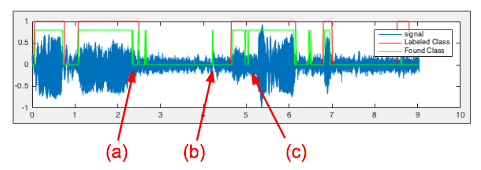
\includegraphics[width=0.6\textwidth]{bilder/smoothing02.png}
	\caption{Klassifizierung vor dem Decision Smoothing}
	\label{img:beforeSmoothing}
\end{figure}

Im Process des \textbf{Decision Smoothing} werden kontextuelle Informationen genutzt, um nachträglich False-Positives und False-Negatives zu entfernen. Es werden dazu die in \cite{vad_entropy} präsentierten Ideen verwendet. Es werden zwei Parameter eingeführt: $\lambda_{min}$, die Mindestlänge einer akzeptierten Cry-Unit, und d$_{min}$, die Mindestlänge eines akzeptierten Stille-Segmentes. Das Decision Smoothing wird nach den folgenden Entscheidungsregeln durchgeführt:

\noindent\rule{\linewidth}{0.3pt}
\begin{itemize}
	\item ist $\lambda (CU_{i}) \leq \lambda_{min}$ ?
	\begin{itemize}
		\item wenn $\lambda (CU_{i-1}) > \lambda_{min}$ und $d (CU_{i-1}, CU_{i}) \leq d_{min}$, dann vereinige $CU_{i}$ mit $CU_{i-1}$ . $\Rightarrow$ behebt False-Negatives des Types (a)
		\item ansonsten entferne $CU_i \Rightarrow$ behebt False-Negatives des Types (b)
	\end{itemize}
	\item wenn $\lambda (CU_{i} > \lambda_{min}$ und $d (CU_{i-1}, CU_{i}) \leq d_{min}$, dann vereinige $CU_{i}$ mit $CU_{i-1}$ . $\Rightarrow$ behebt False-Negatives des Types (c)
\end{itemize}
\noindent\rule{\linewidth}{0.3pt}

Die Entscheidungsregeln greifen Algorithmus greifen nur auf die aktuellen und die letzten bekannte Cry-Unit um, um eine kontinuierliche Analyse zu gewährleisten, weshalb die Entscheidungsregeln jedoch auch komplex sind. Bei einer offline-Analyse können die Entscheidungsregeln vereinfacht werden, da False-Negative Type (a) und (c) mit der selben Regeln abgefragt werden können. Algorithmus \ref{alg:decisionSmoothing} zeigt in Pseudo-Code, wie das Decision-Smoothing durchgeführt wird. Input der Funktion ist die Liste aller Cry-Units $CU_{all}$, die durch Algorithmus \ref{alg:cryUnit} entstanden ist, sowie die Grenzwerte $\lambda_{min}, d_{min}$. Ausgang der Funktion ist die Liste aller Cry-Units nach dem Decision-Smoothing $CU_{smoothed}$.

\begin{algorithm}[H]
	\caption{Decision-Smoothing of VAD}
	\label{alg:decisionSmoothing}
	\begin{algorithmic}[1]
		\Function{decisionSmoothing}{$CU_{all}, \lambda_{min}, d_{min}$}
		\State $CU_{smoothed} \gets[CU_{all}[1]] $
		\For{ $i = 2...length(CU_{all})$}
		\State $cu_i \gets CU_{all}[i]$
		\State $cu_{i-1} \gets CU_{smoothed}[end]$
		\If{$\lambda(cu_i) > \lambda_{min}$}
		\If{d$(cu_{i-1},cu_{i}) > d_{min}$}
		\State $CU_{smoothed} \gets [CU_{smoothed}, cu_i] $
		\Else
		\State \Comment Erase False-Negative Type (c)
		\State $cu_i \gets \text{vereinige}(cu_i, cu_{i-1})$
		\State $CU_{smoothed} \gets [CU_{smoothed}[1:end-1], cu_i] $
		\EndIf
		\Else
		\State \Comment Erase False-Negative Type (a)
		\If{$\lambda(cu_i) > \lambda_{min} \wedge  d(cu_{i-1},cu_{i}) \leq d_{min}$ }
		\State $cu_i \gets \text{vereinige}(cu_i, cu_{i-1})$
		\State $CU_{smoothed} \gets [CU_{smoothed}[1:end-1], cu_i] $
		\Else
		\State \Comment Don't accept $cu_i$. Erases False-Positives (b)
		\EndIf
		\EndIf
		\EndFor
		
		\Return $CU_{smoothed}$
		\EndFunction
		
	\end{algorithmic}
\end{algorithm}

Abbildung \ref{img:after-smoothing} zeigt das Signal vor und nach dem Decision-Smoothing. Die Parameter wurden experimentell mit $\lambda_{min} = 50 ms$ und $d_{min} = 50 ms$ bestimmt.

\begin{figure}[h]
	\centering
	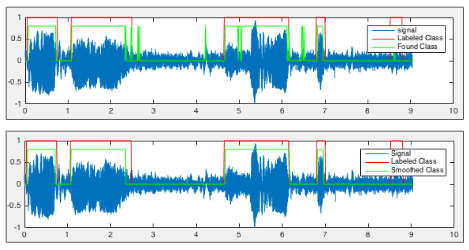
\includegraphics[width=0.6\textwidth]{bilder/smoothing04.png}
	\caption{Klassifizierung vor und nach dem Decision Smoothing}
	\label{img:after-smoothing}
\end{figure}

\section{Segmentierung}
\label{sec:segmenting}
Das Ergebnis der Voice-Activiy-Detection ist eine Liste an Cry-Units  $CU_1 ... CU_n$. Das Ziel ist nun, diese Cry-Units zu Cry-Segmenten zu gruppieren. Ein Cry-Segment definiert sich nach Golub et al \cite{cryModel} als \glqq die komplette klangliche Antwort auf einen spezifischen Stimulus. Sie kann mehrere Cry-Units entahlten \grqq . Die Defintion lässt folgende Fragen offen:

\begin{itemize}[leftmargin=*]
	\item Beginnt das Segment bereits bei Zuführung des Stimulus, oder erst ab der ersten Cry-Unit? 
	\item Wodurch definiert sich der Beginn, wenn ohne Zuführung eines Stimulus das Baby beginnt, zu weinen?
	\item Endet ein Cry-Segment mit Ende der letzten \glqq Cry-Unit\grqq{}, oder erstreckt es sich bis zu Beginn des nächsten Cry-Segmentes?
\end{itemize}

\begin{figure}[h]
	\centering
	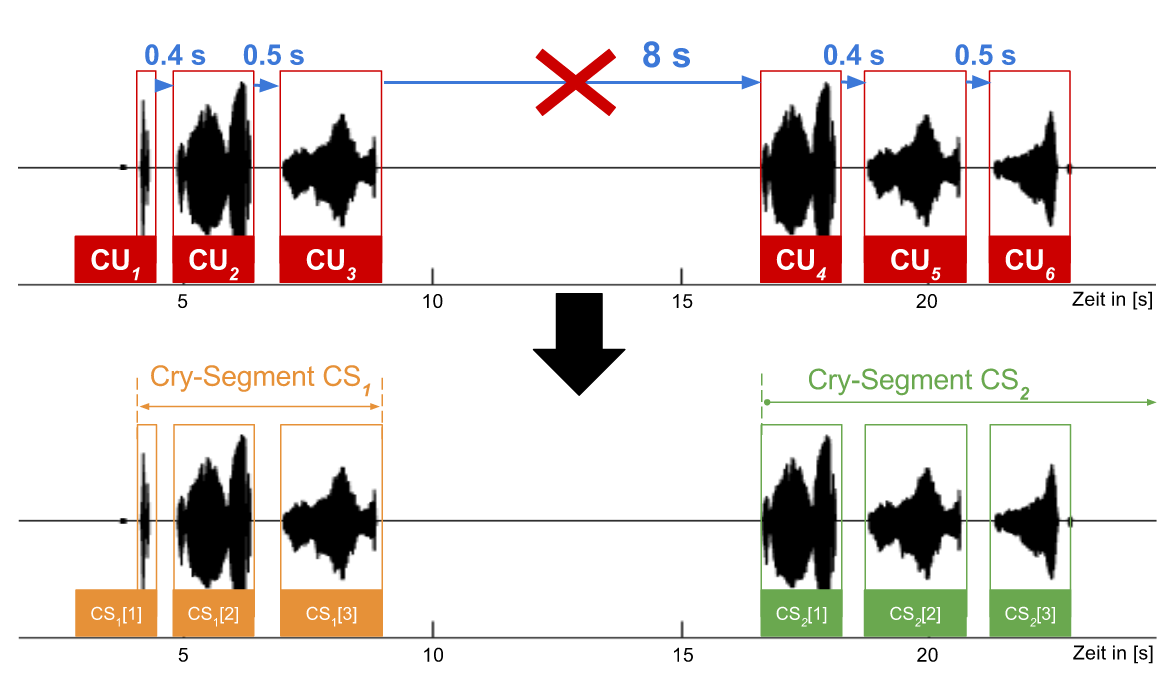
\includegraphics[width=0.75\textwidth]{bilder/segmentierung06.png}
	\caption{Ergebnis der Segmentierung}
	\label{img:segmenting03}
\end{figure}


Die Zusammenfassung von Cry-Units zu Cry-Segmentes unterliegt einer gewissen subjektiven Einschätzung, welche Cry-Units als Zuammengehörig angesehen werden, insbesondere, wenn kein erkennbarer Stimulus vorliegt. Abbildung \ref{img:segmenting02} verdeutlicht das Problem. 

\begin{figure}[H]
	\centering
	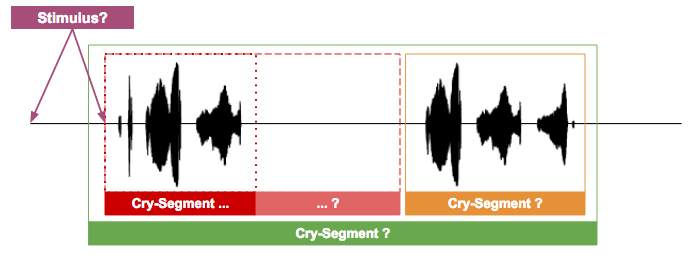
\includegraphics[width=0.48\textwidth]{bilder/segmentierung04.png}
	\caption{Mögliche Segmentierungen eines Signals}
	\label{img:segmenting02}
\end{figure}

Um das Problem zu objektivieren, wird es mathematisch formuliert. 
Eine \emph{Cry-Segment} $[CS]$ wird als Datentyp nach Formel \ref{eq:cry-segment} definiert. Ein Cry-Segment ist folglich eine Liste aufeinander folgenden Cry-Units, die gruppiert werden. Der Start-Zeitpunkt eines Cry-Segmentes wird nach Formel \ref{eq:cry-segment-start} als der Startzeitpunkt der ersten Cry-Unit des Segmentes definiert. Die Begründung für diese Entscheidung liegt darin, dass rein aus dem Audiomaterial der Zeitpunkt des Stimulus nicht festgestellt werden kann und das Segment mit Sicherheit erst bei der ersten feststellbaren Cry-Unit beginnt. Das Ende eines Segmentes wird definiert als das Ende der letzten Cry-Unit nach Gleichung \ref{eq:cry-segment-end}. Die Begründung liegt darin, dass das Ende der Reaktion auf den Stimulus ebenfalls rein aus dem Audiosignal abgeleitet werden kann und somit der einzig feststellbare Indikator die letzte Cry-Unit des Segmentes ist. 

\begin{equation}
CS = [cu_1 ,  ... ,  CU_n]
\label{eq:cry-segment}
\end{equation}

\begin{equation}
start(CS) = CS[1].start
\label{eq:cry-segment-start}
\end{equation}

\begin{equation}
end(CS) = CS[end].end
\label{eq:cry-segment-end}
\end{equation}

Wurde bei der kontinuierlichen Analyse des Signals ein Segment geschlossen, führt die Markierung einer neuen Cry-Unit zur Eröffnung eines neuen Segmentes, dessen Start-Zeitpunkt der Start-Punkt dieser Cry-Unit ist. Die Frage ist, welches Kriterium zum schließen dieses Segments führt. Laut Golub et al \cite{cryModel} ein Cry-Segment \glqq die komplette klangliche Antwort auf einen spezifischen Stimulus \grqq. Eine mögliche und objektiv messbare Interepration dieses Endes ist, dass nach dem Auftreten von Cry-Units eine längere Stille mit einer  Abwesenheit von Cry-Units festgestellt wird, da das Baby \glqq aufgehört hat, zu weinen \grqq. Übertragen auf die in \ref{sec:CryUnit} vorgestellte Terminologie heißt das, dass ein Segment beendet und ein neues begonnen wird, wenn die Distanz (Zeitraum der Stille) zwischen zwei benachbarten Cry-Units d$(CU_{i}, CU_{i+1})$ einen gewissen Grenzwert $t_{seg-max}$ überschreitet. Gleichung \ref{eq:cry-segment-constraint1} formalisiert diesen Zusammenhang. Daraus lässt sich schlussfolgern, dass die Distanzen zwischen allen benachbarten Cry-Unit eines Segmentes unter diesem Grenzwert $t_{seg-max}$ liegen. Gleichung \ref{eq:cry-segment-constraint2} formalisiert diese Nebenbedingung an die Cry-Units eines Segmentes. 

\begin{equation}
d(cu_i, cu_{i+1}) > t_{seg-max} \rightarrow CS_{n} =[CS_n, cu_i] \wedge CS_{n+1} = [cu_{i+1}]  
\label{eq:cry-segment-constraint1}
\end{equation}

\begin{equation}
\forall i = 1 ... \text{length}(CS)-1: \text{d}(CS[i], CS[i+1]) \leq t_{seg-max}
\label{eq:cry-segment-constraint2}
\end{equation}

Die einfachste Art, $t_{seg-max}$ festzulegen, ist, einen festen Grenzwert von $t$ s zuzuweisen. Abbildung \ref{img:segmenting03} visualisiert die so resultierende Segmentierung an einem Beispiel. Jeder Grenzwert mit $t_{seg-max} > \SI{0.5}{\second}$ würde zu der gezeigten Segmentierung führen. 

Algorithmus \ref{alg:crySegment} zeigt die Segmentierung nach diesem Prinzip in Pseudo-Code. Input des Algorithmus ist die Liste aller Cry-Units $CU_{all} = [cu_1 ... cu_n]$, die nach dem Decision-Smoothing nach Algorithmus \ref{alg:decisionSmoothing} entstanden ist.  Das Ergebnis des Algorithmus ist die Liste, die alle gefundene Cry-Segmente  $[cs_1 ...  cs_n]$ enthält. 

\begin{algorithm}[H]
	\caption{Gruppierung von Cry-Units zu Cry-Segments}
	\label{alg:crySegment}
	\begin{algorithmic}[1]
		\Function{segmentCryUnits}{$CU_{all}, t_{seg-max}$}
		\State $ CS_{all} \gets []$
		\State $ cs_i \gets [CU_{all}[1]]$
		\For{ $i = 2...length(CU_{all})$}
		\State $ cu_i \gets CU_{all}[i]$
		\State $cu_{i-1} \gets CU_{all}[i-1]$
		\If{d$(cu_{i-1},cu_i) < t_{seg-max}$}
		\State $cs_i \gets [cs_i , cu_i]$
		\Else
		\State $CS_{all} \gets [CS_{all}, cs_i]$
		\State $cs_i \gets [cu_i]$
		\EndIf
		\EndFor
		\Return $CS_{all}$
		
		\EndFunction
		
	\end{algorithmic}
\end{algorithm}

Algorithmus  \ref{alg:crySegment} kann zwar kontinuierlich durchgeführt werden, da er jeweils nur auf die aktuelle gefundene und eine vergangene Cry-Unit zurückgreift, hat in dieser Form jedoch den nachteil, dass das Ende eines Segmentes später als notwendig festgestellt wird. Angenommen, ein Grenzwert von $t_{seg-max} = \SI{20}{\second}$ wurde festgelegt


Bei einer kontinuierlichen durchgeführten Segmentierung wird das erste Segment dann eröffnet, sobald die erste Cry-Unit durch die VAD markiert wurde, und diese Cry-Unit dem Segment hinzugefügt. Die Dauer der Stille nach dieser Cry-Unit wird kontinuierlich gemessen. Wird ein nächste Cry-Unit festgestellt, bevor die Stille $d_{seg-max}$ übersteigt, so wird diese Cry-Unit dem Segment hinzugefügt und das Messen der Stille nach dieser Cry-Unit beginnt von vorne. Dieser Prozess wird so lange wiederholt, bis die Dauer der Stille nach einer hinzugefügten Cry-Unit $d_{seg-max}$ übersteigt. Dann wird das Segment beendet und der Endzeitpunt des Segmentes auf den Endzeitpunkt der letzten Cry-Unit gesetzt. Abbildung \ref{img:segmenting03} zeigt die resultiderende Segmentierung für Beispielsignal mit $d_{seg-max}  = \SI{3}{\second}$. Tatsächlich würde in dem Beispiel jeder Grenzwert $d_{seg-max} >\SI{0.5}{\second}$ zur gezeigten Segmentierung führen.

Es gibt verschiedene Möglichkeiten, die höchst mögliche Pause d$_{seg-max}$ zu definieren. Der Einfachste Fall, der auch in Abbildung \ref{img:segmenting03} angenommen wurde, ist das Setzen eines global festlegten Grenzwertes. Weitere Möglichkeiten sind, d$_{seg-max}(CS)$ als Funktion des Segmentes selber zu gestalten. So könnte beispielsweise ein längeres Segment eine höhere maximal-Pause erzeugen. 

Schlussendlich konnten in der Fachliteratur keine konkreten Hinweise zur Bestimmung von d$_{seg-max}$ gefunden werden. Daher wurde entschieden, dem Arzt, der das System benutzt, selber einstellen zu lassen. Es wird mit einem Festen 

\section{Feature-Extraction}
\label{sec:segmentFeatures}

\section{Ableitung der Schmerz-Scores}
\label{sec:regressionPainScore}

\section{Visualisierung}
\label{sec:visualisation}